\chapter{Introduction}

\section{Image Segmentation}
Image segmentation is the task of splitting a digital image into one or more regions of interest. It is a fundamental problem in computer vision and many different methods, each with their own advantages and disadvantages, exist for the task. Image segmentation is a particularly difficult task for several reasons. Firstly, the ambiguous nature of splitting up images into objects of interest provides a trade off between making algorithms more generalized or having many user specified parameters. Secondly, imaging artificats such as noise, inhomogeneities, acquisition artifacts and poor contrast, are very difficult to account for in segmentation algorithms without a high level of interactivity from the user. 

In this report, segmentation is discussed in a medical imaging context however the proposed algorithm could equally be used in general purpose segmentations. Segmented images are typically used as the input for applications such as classification, shape analysis and measurement. In medical image processing, segmented images are used for studying anatomical structures, diagnosis and assisting in surgical planning.

Image segmentation also encompasses three dimensional volume segmentations, which are slower to compute by an order of magnitude. It should be noted that before such algorithms existed, segmentation of medical images was done by hand by experts. This was a very accurate, yet slow, process. These segmentations will form the gold standard with which to compare algorithmic segmentations.

In this report, the level set method is used for the purposes of segmentation. Their principal disadvantage is that they are relatively slow to compute, which provides the motivation for optimizing and accelerating such algorithms using graphics processing units (GPUs). Section \ref{upwinding} discusses this further.



\section{Parallel Processing}
The algorithms for processing level sets have vast parallelization potential. Section \ref{levelsetalgorithm} details the algorithms used to discretize the level set equation and Section \ref{parallel} dicusses how these can be executed on graphics hardware.
	\subsection{GPGPU}
General purpose computation on graphics processing units (GPGPU) is the technique of using graphics hardware to compute applications typically handled by the central processing unit (CPU). Graphics cards over the past two decades have been required to become highly efficient at rendering increasingly complex 3D scenes at high frame rates. This has forced their architecture to be massively parallel in order to be compute graphics faster than general purpose CPUs.

Compared to a CPU, a GPU features many more transistors on the control path due to the lower number of control instructions required. Memory is optimized for throughput and not latency, with strict access patterns. GPUs are not optimized for general purpose programs, and does not have the complex instruction sets, or branch control of the modern CPU. It should be noted however that modern CPUs feature multiple cores in order to take advantage of parallel processing. 

The advent of GPGPU programming came with programmable shader units that allowed applying small programs to each pixel or vertex in the rendering pipeline. In order to write code to program the shader units, shading languages had to be used in conjunction with graphics APIs such as DirectX and OpenGL. NVIDIA developed the high-level shading language Cg to assist in programming shaders, however it still required knowledge of graphics APIs. More recently, languages have been developed that allow the programmer to implement algorithms without any knowledge of graphics APIs or architectures. One such language is NVIDIA CUDA, and is the language chosen for the optimizations in this project.

	\subsection{CUDA}
Compute Unified Device Architecture, or CUDA, is NVIDIA's GPGPU technology that allows for programming of the GPU without any graphics knowledge. The C language model has at its core three key abstractions, from \cite{cuda}: a heirarchy of thread groups. shared memories, and barrier synchronization. This breaks the task of parallelization into three sub problems, which allows for language expressivity when threads cooperate, and scalability when extended to multiple processor cores.

		\subsubsection{Framework}
CUDA uses extends C by allowing a programming to write \textit{kernels} that when invoked execute a thousands of lightweight identical threads in parallel. CUDA arranges these threads into a hierarchy of blocks and grids, as can be seen in Figure \ref{fig:cudathreads} allowing for runtime transparent scaling of code to different GPUs. The threads are identified by their location within the grid and block, making CUDA perfectly suited for tasks such as image processing where each threads is easily assigned to an individual pixel or voxel.

\begin{figure}[p]
	\centering
		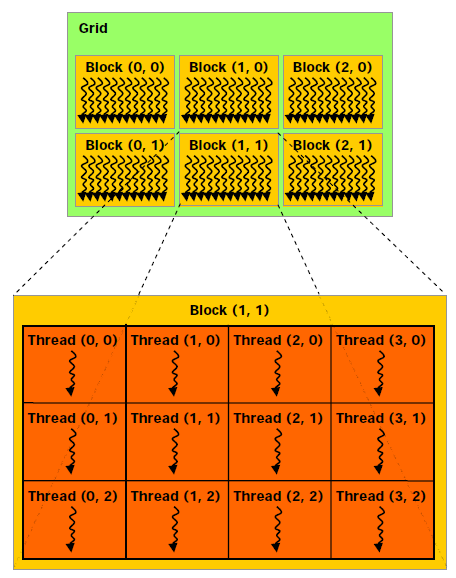
\includegraphics[scale=0.4]{images/cudathreads.PNG}
		\caption{A grid of thread blocks. This figure is taken from \cite{cuda}}
	\label{fig:cudathreads}
\end{figure}

When writing and optimizing complex parallel code in CUDA it is often found that threads may need to cooperate. The memory hierarchy of CUDA threads is shown in Figure \ref{fig:cudamemory}. Here it can be seen that each thread has access to: a per-thread private local memory, a per-block on-chip shared memory to share data between threads, and finally an off-chip global memory accessible to all threads within all blocks. There are also constant and texture memory spaces accessible to all threads, however these are not featured in our algorithm and so will not be discussed in any further detail.

\begin{figure}[p]
	\centering
		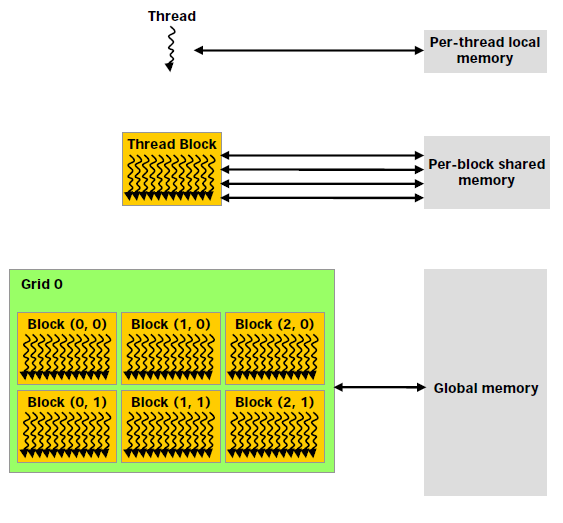
\includegraphics[scale=0.4]{images/cudamemory.PNG}
		\caption{The memory hierarchy of CUDA threads and blocks. This figure is taken from \cite{cuda}}
	\label{fig:cudamemory}
\end{figure}

		\subsubsection{Performance Guidelines}
There are many techniques to optimize a parallel algorithm. Firstly, the optimum block and grid sizes should be used to ensure maximum `occupancy'. Occupancy is the ratio of the number of active warps (32 parallel threads) to the maximum number of active warps supported by the GPU multiprocessor. To maximise efficiency, there is a trade off between making the occupancy very high, ensuring no multiprocessor is ever idle, and making it low enough to ensure no bank conflicts.

Secondly, one of the best ways in which to optimize the parallelization is through efficient memory usage. The global memory space is not cached and therefore has a much higher latency and lower bandwidth than on-chip shared memory. Therefore it is the aim of the programmer to minimise global memory accesses. From \cite{cuda}, it recommended that each thread in a block firstly loads data from global memory to shared memory, synchronizes with all other threads within the thread block to ensure shared memory locations have been written to, processes the data, synchronizes again to ensure shared memory has been fully updated with results, and finally writes the results back to global memory coalesced.

\textit{Coalescence} is an important concept in memory management as it can speed up memory reads and stores significantly. \cite{cuda} lists the following three conditions for coalescing: ``threads must access either 32-bit words, 64-bit words, or 128-bit words'', ``all 16 words must lie in the same segment of size equal to the memory transaction size'' and ``threads must access the words in sequence''. Devices of higher \textit{compute capability} feature incremental improvements to the core architecture, such as more relaxed requirements for coalescence (or support for double-precision floating point accuracy).